%\section{Introduction}

\section{Estimation and Construction of the Policy Forecasts}
\label{sec:method}

\subsection{Data}
%Put the description of the data here, since we already talk about the scenarios afterwards.
The data used for this study was taken from \citet{morita2017}. It contains quarterly data on government spending, excess stock returns, GDP, CPI inflation, private consumption, and non-residential investment from 1980 (Q1) to 2015 (Q2). Government spending, GDP, consumption and investment were provided as real seasonally adjusted series, which were converted into per capita values. \citeauthor{morita2017} calculated CPI inflation using a X-12 ARIMA model for seasonal adjustment on the year-on-year inflation rate, which was then converted into a quarterly series by taking the average of three months. Quarterly inflation was then calculated through the log differences of the obtained values. For calculating the excess stock returns of the construction sector, \citeauthor{morita2017} followed~\citet{fisher2010} by translating monthly data on the growth rate of stock prices and subtracting the returns of the market as a whole from the construction industry returns.

\subsection{Robustness Checks and Model Calibration}

In a first step, estimations employing a VAR in levels were made. The selection of the forecast models was conducted mainly based on statistical criteria. The preferred criteria for lag order selection were the Akaike Information Criterion (AIC) and the Final Forecast Prediction Error (FPE), since the main objective was to optimize our forecast. The model was estimated using the presample period from 1980 Q1 to 2013 Q2, giving us $T=133$ observations over time for estimation. The deterministic terms tested for model selection were an intercept, a time trend, and - following \cite{morita2017} - a quadratic time trend. For the subset model selection, we also employed the System SER method for searching subset model restrictions to optimize the AIC. In our exercise, however, restricted models in levels produced inferior forecasts compared to unrestricted models. The only restriction which was added was a zero restriction on the quadratic trend for investment, since this effect tended to lead to the forecasts drifting off the realized values in a negatively quadratic fashion. Concerning structural stability, the CUSUM test indicated that the estimated process was structurally stable in all tested settings.

For the differenced VAR model, we took a similar approach to model selection. We differenced the time series of GDP, investment and consumption in logs in the period between 1980 Q1 and 2013 Q2. For the endogenous variables in the differenced VAR model, both the AIC and the FPE suggested a lag order of $p=3$. For government expenditure, a lag order of $q=1$ was chosen. The results were contrasted with models employing a higher exogenous lag order. The residual autocorrelation plot in Figure~\ref{fig:autocorr_diff} shows no significant autocorrelation in the residuals for all endogenous time series. The resulting baseline forecasts plotted together with the actual values of the time series can be seen in Figure~\ref{fig:baseline_comp_diff}. The forecasts manage to capture all data points within their forecast bands, except for the investment growth in the fourth quarter of 2013. For the differenced VAR model, no deterministics were included, since the series were difference-stationary and hence did not exhibit trends or shifts.

%The specification of the dVar model was done analogously to the model specification in levels. As described, we differenced the time series of GDP, investment and consumption in logs in the period between 1980 Q1 and 2013 Q2. Again AIC and FPE suggested an endogenous lag order of 3 for the dVar model. For the dVar model, the suggested lag order was used, as it yielded superior results with regard to autocorrelation and forecast power when compared to the dVar(4) model case. Figure~\ref{fig:autocorr_diff} also shows that the model shows no serial autocorrelation up until the ninth lag. Also, no deterministics were included for the dVar(3) model, as the differenced time series did not exhibit trends or shifts.  



%The approach of this exercise is similar to~\cite{kapeta12} [Kapetanios et al. (2012)]. For assessing the potential impact of a change in government spending, we will examine conditional forecasts. In a first step, the following VAR(p) model in its general form allows us to get forecasts and impact estimations in levels: 
%
%\begin{equation}
%y_{t} = \sum^{p}_{i = 1}A_{i}y_{t-i} + Cd_{t} + \sum^{q}_{j=1}B_{j}g_{t-j} + u_{t}
%\end{equation} 

%where $y_{t}$ is a vector containing quarterly data on GDP, investment, excess stock returns of the construction sector, consumption, and CPI inflation\footnote{[Review Comment]: In the theoretical part preceding this section, I will explain why we include the excess stock returns at all.}, $d_{t}$ is a vector of determinants, such as potential trend terms and intercepts to be included in the model, and $g_{t-j}$ is a vector containing exogenous government expenditure in the $(t-j)^{\text{th}}$ period. Thus, $p$ gives us the endogenous lag order, while $q$ indicates the number of exogenous lags to be included in the model. 
%
%In addition to the forecasts in levels, we will also use a 
%differenced VAR model (dVar), to examine the potential impact of government expenditure on the growth paths of our variables of interest:

%\begin{equation}
%\ln\left(\frac{y_{t}}{y_{t-1}}\right) = \sum^{p}_{i = 1}\left[A^{*}_{i}\ln\left(\frac{y^{\ast}_{t-i}}{y^{\ast}_{t-i-1}}\right) + Z_{i}x_{t-i}\right]  + Cd_{t} + \sum^{q}_{j=1}B_{j}g_{t-j} + u_{t}
%\end{equation}
%
%Where $y_{t-i}^{\ast}$ now contains our variables of interest, except those, that are already given in log-differences. In our case, these are the excess stock returns and CPI inflation. These are collected in $x_{t-i}$.
%Aside from allowing us to examine the effects of government expenditure on the growth paths of our variables, adding a differenced version of our original VAR model also serves as a robustness check against potential cointegration of degree $I(1)$.

\subsection{Construction of the Policy Counterfactuals}

As the time series on CPI is stationary and the other time series are difference-stationary, we decided for a VAR model in differences taking the log differences of all variables except for CPI, which is already constructed as log-differences over time, and government spending, which we want to control directly to contrast the counterfactual scenarios. By doing so, the impact on the endogenous variables can be interpreted in terms of growth rates. The transformation of the series on excess stock returnshad to be adjusted, as it contained negative values. To circumvent this problem, the neglog transformation as proposed by \citet{whittaker2005} was applied:

\begin{equation}
\text{nl}(x) = 
\begin{cases}
-\ln(-x + 1) & x \leq 0 \\
\ln(x + 1) & x > 0
\end{cases}
\end{equation}



Although estimating a VAR in differences rather than imposing cointegration relationships by employing a VECM model can lead to loss of information due to the "differencing out" of relationships, the focus of this study is to optimize the model with respect to forecasting power, for which \citet{duy1998modeling} found that VAR models in differences perform well. Thus, for the estimation of the policy forecasts, the following VAR model is considered

\begin{equation}
\Delta y_{t}= \sum^{p}_{i = 1}A_{i}\Delta y_{t-i} + \sum^{q}_{j=0}B_{j}g_{t-j} + u_{t}
%\sum^{p}_{i = 1}\left[A_{i}(\ln(y_{t-i}) - \ln(y_{t-i-1})) + C_{i}\pi_{t-i}\right] + \sum^{q}_{j=0}B_{j}g_{t-j} + u_{t}
\end{equation}

where $y_{t}$ is a vector containing the endogenous variable in their transformation as described above\footnote{Note that the CPI series is, by its construction, already a differenced time series. Hence, strictly speaking,  $y_{t}$ contains the price level.}, $g_{t-j}$ is a vector containing exogenous government expenditure in the $(t-j)^{\text{th}}$ period. Thus, $p$ gives us the endogenous lag order, while $q$ indicates the number of exogenous lags to be included in the model. 

Another reason for choosing a differenced VAR model ties in with the discussion mentioned in Section~\ref{sec:litrev}. The methodology employed by \citeauthor{lenza2010} and \citeauthor{kapetanios2012}, on the offer the practical advantage that they require \emph{reliability of the produced forecasts} imposing only little structure on the data. In such cases, \citeauthor{duy1998modeling} showed that differenced VAR models perform similarly well as error-correction models with theoretical and estimated conintegration restrictions. The strongest assumptions we make for this model are the ordering of the variables in question and the exogeneity of government spending.

Using this model, we will construct five different forecast scenarios. First, we will estimate one baseline scenario, where the exogenous government expenditure will be the same as the actually realized levels after our pre-sample period. The baseline forecasts will serve as a benchmark for evaluating the effects we observe, when we change government expenditure for our alternative scenarios. Then, we consider the following four different policy paths:

\begin{enumerate}
	\item	A proportional increase over the forecast horizon: We will consider a scenario, in which government spending is 10\% (Scenario 1) and 25\% (Scenario 2) higher in each quarter than it actually was in the respective quarter.
	\item	A constant increase over time: In this scenario, we will keep the increase of government spending equal with respect to Scenario 1 a and b by dividing the overall increase over the forecast period by the length of the forecast period. This way we increase government spending in each period by the same amount in absolute terms.
	\item	A one-time increase in the first period with an instant "payback": For this scenario, we will assume a government spending increase of 10\% (Scenario 1) or 25\% (Scenario 2) in the first forecast period, after which government spending will immediately return to its actually realized values.
	\item	A one-time increase with constant "payback": Similar to the one-time increase, we assume government spending to increase by 10\% or 25\% in the first period. Instead of immediately going back to the original levels of government spending, however, we assume that the government decreases government spending by a constant amount such that the economy reaches the baseline level of expenditure at the end of the forecast horizon.
\end{enumerate}

To assess whether the forecasts differ statistically from the baseline, we use the Wilcoxon signed-rank test, following \citet{franses1991}, as the Jarque-Berra test indicated that the normality assumption is violated. 



%\begin{figure}[ht]
%	\centering
%		\includegraphics[scale=0.7]{scenariopaths.jpg}
%	\caption{The government expenditure paths used for the construction of the policy counterfactuals.}
%	\label{fig:scenariopaths}
%\end{figure}


%\subsection{Robustness Checks and Model Calibration}
%
%The selection of the forecast models was conducted mainly based on statistical criteria. The preferred criteria for lag order selection were the Akaike Information Criterion (AIC) and the Final Forecast Prediction Error (FPE), since the main objective was to optimize our forecast. The model was estimated using the presample period from 1980 Q1 to 2013 Q2, giving us $T=131$ observations over time for estimation.

%\subsubsection{VAR in Levels}
%
%The deterministic terms to be included in the model in levels were an intercept, a time trend, and - following \cite{morita17}[Morita 2017] - a quadratic time trend. Furthermore, government expenditure was added as an exogenous variable, so that we could freely adjust it for our scenarios after the pre-sampling period\footnote{[Review Comment]: I also thought about explaining it by some economic intuition, since to me, it seems plausible that economic variables three or four periods ago might influence the decision making of policy makers, but I doubt that the share of government spending is being directly and - more or less - "mechanically" determined by those variables through causation and in a system of equations is really large.}. For the subset model selection, we also employed the System SER method for searching subset model restrictions to optimize the AIC. In our exercise, however, restricted models produce inferior forecasts compared to unrestricted models. The only restriction which was added was a zero restriction on the quadratic trend for investment, since this effect tended to lead to the forecasts drifting off the realized values in a negatively quadratic fashion. The restricted model was then estimated using estimated generalized least squares (EGLS).
%
%Concerning structural stability, the CUSUM test indicated that the estimated process was structurally stable in all settings. A reason for concern, however, was serial autocorrelation in the error terms of consumption and CPI inflation on the fourth lag. Seasonal dummies were insignificant for all our variables and including them did not mitigate the problem. Thus, instead of the VAR(3) model, which was suggested by AIC and FPE, a fourth endogenous lag was included. Figure~\ref{fig:autocorr_simple} shows the result of fitting a VAR(4) model. After increasing the lag order, autocorrelation only occured on later lags, except for consumption, for which serial autocorrelation on the fourth lag was barely significant. 
%
%For government expenditure an exogenous lag order of 1 was chosen. The baseline forecasts resulting from this model in comparison with the realized values after the presample period can be seen in Figure~\ref{fig:baseline_comp_simple}. In general, the predictions of our (given by the marked line) model seemed to produce viable forecasts, as the realized values after 2013 Q2 lie within our confidence intervals. However, there are two exceptions. Consumption in Japan has seen a sharp decline from the first to the second quarter of 2014. This coincides with the consumption tax hike from 5\% to 8\%, which came into effect in April 2014 and is likely to have caused the sudden shift in consumption. [Add reliable source here.]  This could also have been the cause for the more steady decline in CPI inflation between the beginning of 2014 and 2015\footnote{[Review Comment]: Also, there has been a revision of the calculation method for the CPI inflation and a reset of the calculations between January 2015 and June 2016. I will look into whether this might have played a role too, and whether Morita has also accounted for the base change, if it was relevant.}
%
%\begin{figure}[ht]
%	\centering
%		\includegraphics[scale=0.4]{autocorr_simplevar_setting1.jpg}
%	\caption{Autocorrelation for the VAR(4) model.}
%	\label{fig:autocorr_simple}
%\end{figure}
%
%\begin{figure}[ht]
%	\centering
%		\includegraphics[scale=0.5]{Baseline_comp_simple.jpg}
%	\caption{Baseline forecasts for the endogenous variables of the VAR(4) model.}
%	\label{fig:baseline_comp_simple}
%\end{figure}

%\subsubsection{dVar Model}

%For the endogenous variables, both the AIC and the FPE suggested a lag order of $p=3$. For government expenditure, a lag order of $q=1$ was chosen. The residual autocorrelation plot in Figure~\ref{fig:autocorr_diff} shows no significant autocorrelation in the residuals for all endogenous time series. The resulting baseline forecasts plotted together with the actual values of the time series can be seen in Figure~\ref{fig:baseline_comp_diff}. The forecasts manage to capture all data points within their forecast bands, except for the investment growth in the fourth quarter of 2013. 
%The specification of the dVar model was done analogously to the model specification in levels. As described, we differenced the time series of GDP, investment and consumption in logs in the period between 1980 Q1 and 2013 Q2. Again AIC and FPE suggested an endogenous lag order of 3 for the dVar model. For the dVar model, the suggested lag order was used, as it yielded superior results with regard to autocorrelation and forecast power when compared to the dVar(4) model case. Figure~\ref{fig:autocorr_diff} also shows that the model shows no serial autocorrelation up until the ninth lag. Also, no deterministics were included for the dVar(3) model, as the differenced time series did not exhibit trends or shifts.  

\begin{figure}[h]
	\centering
		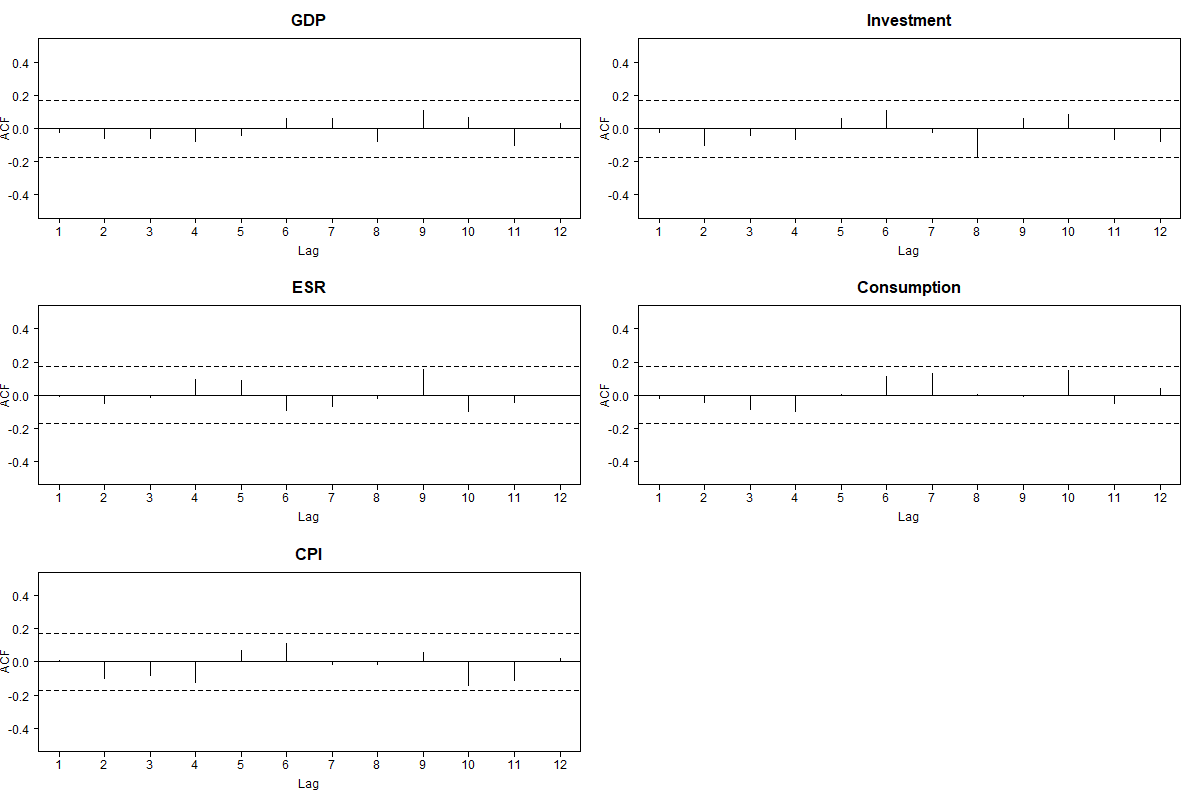
\includegraphics[width=1\textwidth,height=1\textheight,keepaspectratio]{acfplot.png}
	\caption{Autocorrelation for the VAR(3) model in log differences.}
	\label{fig:autocorr_diff}
\end{figure}



% The baseline forecasts in this case caputre all the realized values within their confidence intervals, except for the drop in consumption in the second quarter of 2014 discussed above.


\begin{figure}[ht]
	\centering
		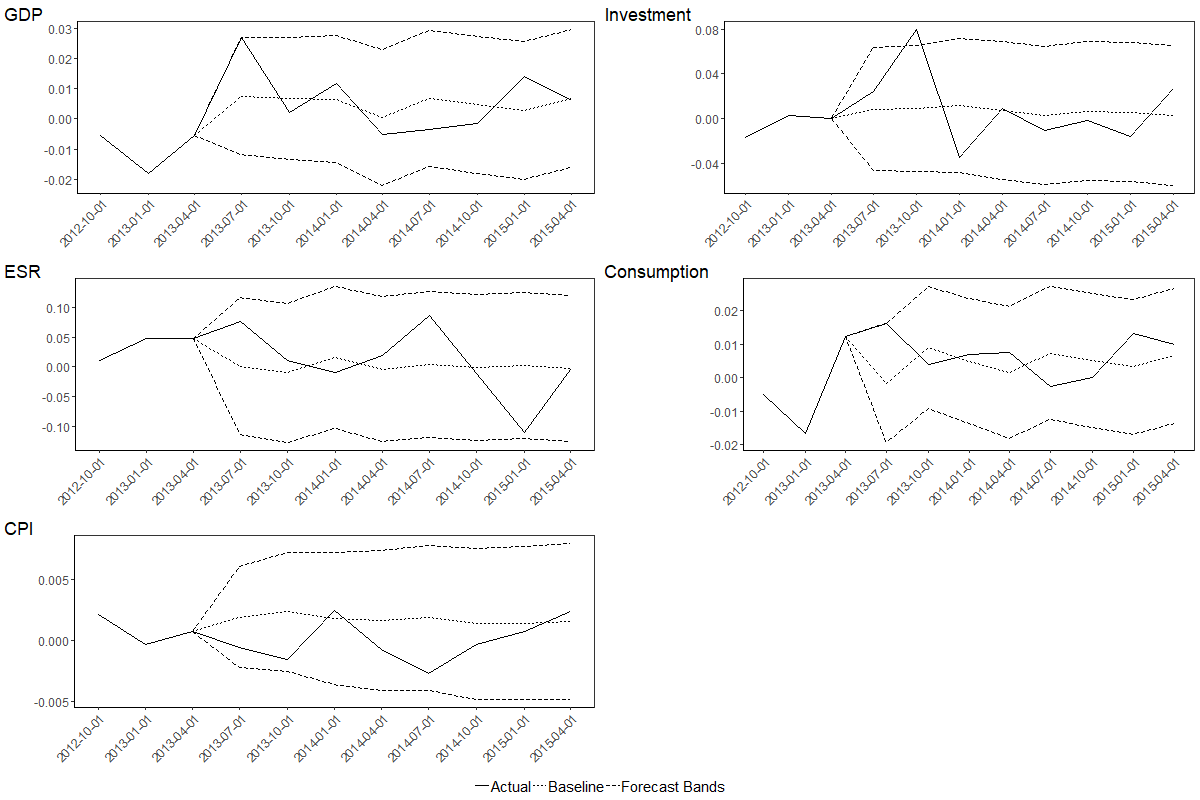
\includegraphics[width=1\textwidth,height=1\textheight,keepaspectratio]{basefcst.png}
	\caption{8-step forecasts for the baseline scenario.}
	\label{fig:baseline_comp_diff}
\end{figure}

